\section{Introduction}
\label{sec:introduction}

\IEEEPARstart{S}{imulation} of multibody systems with frictional contact has
proven indispensable in robotics, aiding at multiple stages during the
mechanical and control design, testing, and training of robotic systems.
Robotic applications often require robust simulation tools that can perform at
interactive rates without sacrificing accuracy, a critical prerequisite for
meaningful sim-to-real transfer. However, reliable modeling and simulation
through contact remains somewhat elusive.

Rigid body dynamics with frictional contact is complicated by the non-smooth
nature of the solutions. It is well known \cite{bib:baraff1993issues} that rigid
contact when combined with the Coulomb model of friction can lead to paradoxical
configurations for which solutions in terms of accelerations and forces do not
exist. These phenomena are known as Painlev\'e paradoxes
\cite{bib:hogan2017regularization}.
%
\begin{figure}[!ht]
	\centering
    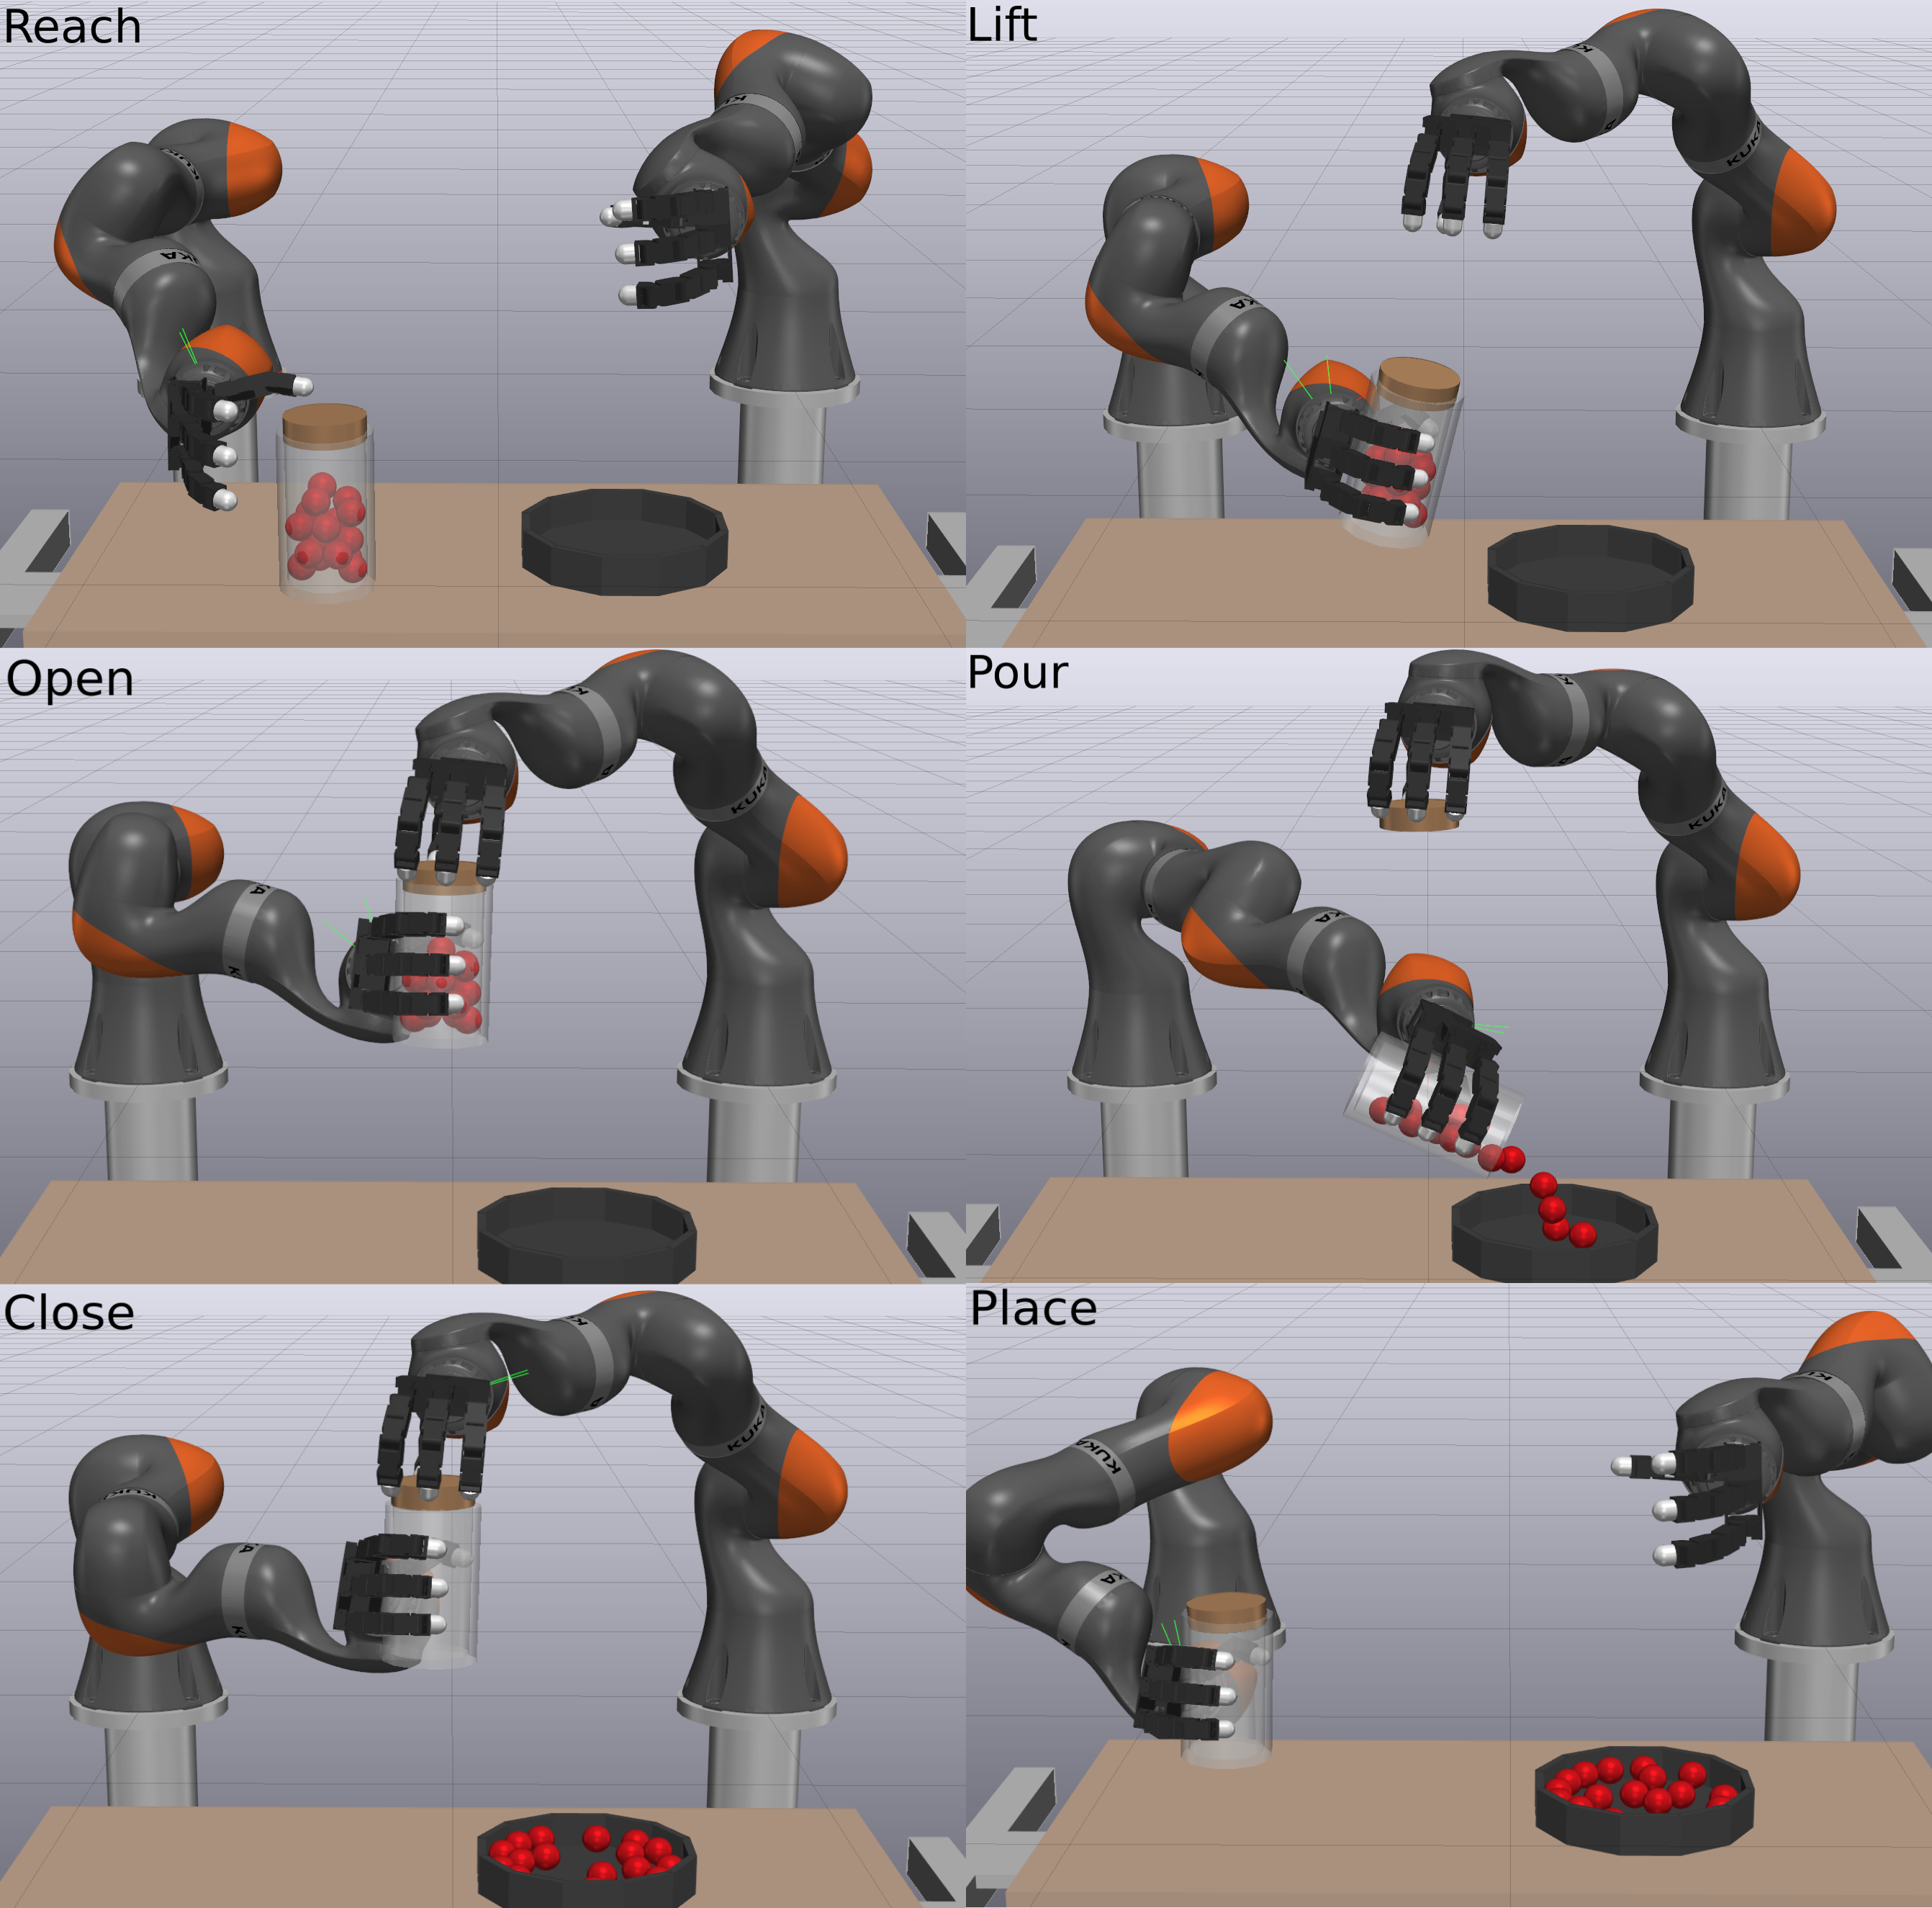
\includegraphics[width=0.95\columnwidth]{figures/dual_arm/tiled.png}
	\caption{\label{fig:dual_arm_frames}
    Keyframes of a dual arm manipulation task in simulation. The robot is commanded to pick up a jar full of marbles, open it, pour its contents into a bowl, close the lid and place the empty jar back in place. This is a computationally intensive simulation with 148 degrees of freedom and hundreds of contact constraints per time step, see Fig. \ref{fig:dual_arm_contacts}. Our SAP solver is robust and warm-starts effectively, enabling this simulation at interactive rates.}
\end{figure}
%
Theory resolves these paradoxes by allowing
discrete velocity jumps and impulsive forces, formally casting the problem as a
differential variational inequality \cite{bib:pang2008differential}. In practice,
event based approaches can resolve impulsive transitions \cite{bib:haug1986},
though it is not clear how to detect these events even for simple one degree of
freedom systems \cite{bib:hogan2017regularization}.

Nevertheless, the problem can be solved in a weaker formulation at the velocity
level using a time-stepping scheme where the next step velocities and impulses
are the unknowns at each time
step \cite{bib:stewart1996implicit, bib:anitescu1997}. These formulations lead
in general to a non-linear complementarity problem (NCP) or to a linear
complementarity problem (LCP) when a polyhedral approximations of the friction
cone is used. Even though LCP formulations guarantee solution existence
\cite{bib:anitescu1997, bib:stewart1998convergence}, solving them accurately and
efficiently has remained difficult in practice. This has been explained
partly due to the fact that these formulations are equivalent to nonconvex problems
in global optimization, which are generally NP-hard \cite{bib:Kaufman2008}.
Indeed, popular direct methods based on Lemke's pivoting algorithm to solve
LCPs may exhibit exponential worst-case complexity \cite{bib:baraff1994fast}. Similar
to direct methods, popular iterative methods based on projected
Gauss-Seidel (PGS) \cite{bib:duriez2006_realistic_haptic_rendering, bib:bullet}
have also shown exponentially slow convergence \cite{bib:erleben2007velocity}.
These observations are not just of theoretical value, but in practice,
these methods are numerically brittle and lack robustness when tasked with computing contact forces.
This inherent lack of stability and robustness is tackled in software with a
large amount of non-physical constraint softening and stabilization.
Still, the resulting simulation requires a significant amount of bespoke parameter tuning.

To improve computational tractability, Anitescu introduced a \textit{convex
relaxation} of the contact problem \cite{bib:anitescu2006}. This relaxation is a
convex approximation with proven convergence to the solution of a measure
differential inclusion as the time step goes to zero. For sliding contacts,
the convex approximation introduces a \emph{gliding} artifact at a distance $\phi$
proportional to the time step size $\delta t$ and to the sliding velocity
$\Vert\vf{v}_t\Vert$ \cite{bib:mazhar2014}, i.e. $\phi\sim \delta
t\Vert\vf{v}_t\Vert$. The approximation is exact for sticking contacts,
and it can be adequate for robotics applications for which the product $\delta
t\Vert\vf{v}_t\Vert$ is usually sufficiently small. For trajectory optimization,
Todorov \cite{bib:todorov2011} introduces regularization into Anitescu's
formulation in order to write a strictly convex formulation with a unique,
smooth and invertible solution. For simulation, Todorov \cite{bib:todorov2014}
uses regularization to introduce \emph{numerical compliance} that provides
Baumgarte-like stabilization and avoids constraints drift. As a side effect, the
regularized formulation can lead to a noticeable non-zero slip velocity even
during stiction \cite{bib:simbenchmark}.

Even though these formulations introduce a tractable approximation of frictional
contact, they haven't become a popular approach in practice. We
believe this is not because the approximation is not suitable for robotics
applications, but rather because of the lack of robust solution methods with a
computational cost suitable for real-time simulation. Software such as ODE
\cite{bib:ode}, Dart \cite{bib:dart} and Vortex \cite{bib:vortex} use a
polyhedral approximation of the friction cone leading to an LCP formulation.
Algoryx \cite{bib:algoryx} uses a \emph{split solver}, reminiscent of one
iteration in the staggered projections method \cite{bib:Kaufman2008}. Drake
\cite{bib:drake} solves compliant contact with regularized friction with its
transition aware solver TAMSI \cite{bib:castro2020}. 

To our knowledge, Chrono \cite{bib:hrono2016} and Mujoco
\cite{bib:mujoco} are the only software that implement the convex approximation
of contact. The multi-physics simulation package Chrono implements a variant of
the PGS method for solving Anitescu's convex formulation \cite{bib:tasora2011}.
This method is specially targeted to the simulation of very large scale systems
as those found in granular flow. Even though some convergence guarantees are
provided in \cite{bib:anitescu2010}, the solver exhibits low convergence rates.
This is expected for such first order method. Mujoco is a software targeted to
robotics that implements both a PGS solver variant \cite{bib:todorov2014} and a
second order Newton solver. However, the underlying technology is proprietary and
implementation details are not known in the community.

Summarizing, 15 years after the introduction of these convex
approximations, robust and performant algorithms for their solution in practice
are lacking. It is not even clear in the community if these formulations present
a real advantage when compared to more traditional approaches and whether the
artifacts introduced by the approximation are appropriate for robotics
applications. In this work, we aim to provide answers to these questions. 

We make a number of novel contributions. To address accuracy and model validity,
Section \ref{sec:physical_intuition} provides compact expressions for the
impulses that correspond to the optimal velocities of the convex approximation.
This provides intuition for the approximation, even to those without
optimization expertise. Moreover, the artifacts introduced by the approximation
become apparent and can be characterized precisely. In particular,
\emph{regularization terms} introduced by Todorov \cite{bib:todorov2014} (for
Baumgarte-like stabilization) are given a clear physical interpretation. Such
interpretability  allows us to incorporate not only compliant point contact, but
also complex models of compliant surface patches \cite{bib:elandt2019pressure},
as we demonstrate in Section \ref{sec:slip_control}. We introduce in Section
\ref{sec:discrete_time_formulation} a time stepping approach based on the
$\theta\text{-method}$. This includes the popular symplectic Euler method and
the implicit midpoint rule. In Section \ref{sec:spring_cylinder} we demonstrate
that the midpoint rule can achieve second order accuracy even in problems with
frictional contact.

Unlike previous work \cite{bib:anitescu2010,bib:todorov2014} that formulate the
problem in impulses, we write a primal formulation of compliant contact
in velocities (Section \ref{sec:primal_formulation}). We then analytically eliminate constraints from this
formulation to obtain an unconstrained convex problem (Section \ref{sec:unconstrained_convex_formulation}).
To solve this formulation, we develop SAP---the Semi-Analytical Primal  solver---in Section \ref{sec:sap_solver} and study its theoretical and practical
 convergence.  Crucially, we show that SAP warm-starts effectively
using the previous time-step velocities, enabling simulation at real-time rates.  We provide full details needed for implementation,
including formulae for selecting a search direction,
a line search procedure, and sparsity analysis. Section
\ref{sec:understanding_model_parameters} presents 
 regularization procedures that improve numerical
 conditioning without sacrificing the accuracy needed
 for simulation of stiction and simulation of \emph{near-rigid} objects.
This is critical for the simulation of demanding robotics tasks such as
manipulation. We evaluate the accuracy, robustness and performance of SAP
against available commercial and open-source optimization solvers. In Section
\ref{sec:test_cases}, we demonstrate the effectiveness of our approach in a
number of simulation cases, including the simulation of a challenging dual arm
manipulation task. We conclude our work with a discussion on extensions and
variations in Section \ref{sec:variations_and_extensions} and provide
conclusions and future research directions in Section
\ref{sec:future_directions}.
